\subsection{Planeación}

En esta etapa, se estableció el propósito general de la investigación y se definieron las metas, así como las preguntas de investigación, métricas, criterios de clasificación, criterios de inclusión/exclusión y criterios de calidad de los estudios. Ver Figura~\ref{fig:etapa1}.\\

\begin{figure}[htbp]
    \centering
    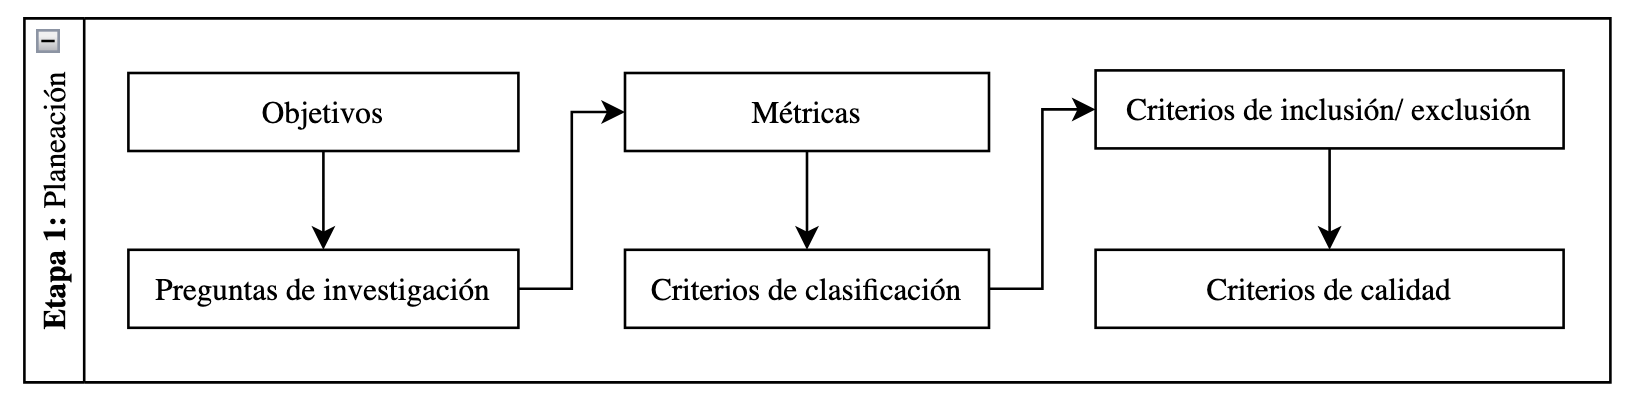
\includegraphics[width=0.8\textwidth]{resources/images/planeacion/etapa1.png}
    \caption{Composición de la etapa de planeación}\label{fig:etapa1}
\end{figure}
\subsubsection{Objetivos}
Teniendo en cuenta los aspectos descritos en la sección de motivación, se definieron 2 metas generales para la revisión sistemática de la literatura que se presentan en el cuadro~\ref{tab:metas}.

\begin{table}[H]
    \centering
    \begin{tabular}{>{\centering\arraybackslash}m{1cm} >{\arraybackslash}m{7cm}}
        \hline
        \textbf{Goal} & \textbf{Description} \\
        \hline
        M1 & Identificar trabajos relacionados con VBC en proyectos de docencia, investigación y extensión. \\
        \\
        M2 & Clasificar trabajos relacionados con VBC en los dominios de desarrollo de software, pensamiento computacional, computación paralela, análisis de datos, inteligencia artificial, redes computacionales, infraestructura de TI, HPC, entre otros. \\
        
        \hline
    \end{tabular}
    \caption{Metas del estudio}\label{tab:metas}
\end{table}

\subsubsection{Pregunta de investigación}

Este modelo permite establecer los aspectos de ``Población'', ``Intervención'', ``Comparación'', ``Salida'' y ``Contexto'' que sirven para situar el trabajo a realizar. Ver Tabla~\ref{tab:PICOC}.
Teniendo en cuenta el modelo PICOC, se definieron las preguntas de investigación. Ver cuadro~\ref{tab:preguntas}.

\begin{table}[H]
    \centering
    \begin{tabular}{>{\centering\arraybackslash}m{0.25\columnwidth} >{\arraybackslash}m{0.70\columnwidth}}
        \hline
        \textbf{Aspecto} & \textbf{Descripción} \\
        \hline
        Población & Trabajos relacionados con la VBC aplicadas en diversos dominios de TI con un énfasis en la educación, investigación y extensión. \\
        \\
        Intervención & Identificación y clasificación de los trabajos en VBC en los dominios de TI establecidos. \\
        \\
        Comparación & 
        1. Se comparan los proyectos que han hecho uso de la VBC para determinar cuáles han tenido mayor tasa de éxito expresado por los autores en cada dominio de TI. \newline
        2. Se analiza el impacto de la VBC en proyectos de docencia, investigación y extensión en comparación con otras soluciones tecnológicas. \\
        \\
        Salida & Estructura de clasificación de los trabajos relacionados con las VBC en cada dominio de TI que han impactado en proyectos de docencia, investigación y extensión. \\
        \\
        Contexto & Docencia, investigación y extensión con apropiación de los dominios de TI en forma de VBC. \\
        \\
        \hline
    \end{tabular}
    \caption{Aspectos del modelo PICOC}\label{tab:PICOC}
\end{table}

\begin{table}[H]
\centering
\caption{Preguntas de investigación y su motivación}
\renewcommand{\arraystretch}{1.4}
\begin{tabularx}{\textwidth}{>{\hsize=0.5\hsize}X >{\hsize=0.6\hsize}X >{\hsize=1.5\hsize}X >{\hsize=2\hsize}X}
\toprule
\textbf{Meta} & \textbf{Pregunta} & \textbf{Descripción} & \textbf{Motivación} \\
\midrule
G1 & Q1 & ¿Cuáles son los trabajos relacionados con tecnologías de virtualización basadas en contenedores (VBC) que podrían impactar positivamente proyectos de docencia, investigación y extensión? & La transversalidad que ofrece la VBC, gracias a su reproducibilidad de entornos, permite estimular diferentes aristas de la sociedad. Su naturaleza facilita el transporte de soluciones de TI entre diferentes entornos, generando que una innovación en cualquier dominio social impacte directamente en otro. \\
\midrule
G2 & Q2 & ¿Cuáles son los principales trabajos relacionados con las tecnologías de virtualización basadas en contenedores (VBC) que podrían contribuir en los diversos dominios de TI, entre los que pueden ser desarrollo de software, pensamiento computacional, computación paralela, análisis de datos, inteligencia artificial, redes computacionales, infraestructura de TI, HPC, entre otros? & Se busca proporcionar una base sólida para investigadores, docentes y profesionales interesados en comprender el estado del arte actual en relación con las VBC, además del alcance y las aplicaciones de estos trabajos sin necesidad de un análisis profundo. \\
\bottomrule
\end{tabularx}\label{tab:preguntas}
\end{table}

\subsubsection{Métricas}

Texto por agregar...

\subsubsection{Tópicos de investigación}

Texto por agregar...

\subsubsection{Criterios de inclusión y exclusión}

Texto por agregar...

\subsubsection{Criterios de calidad}

Texto por agregar...